
%(BEGIN_QUESTION)
% Copyright 2010, Tony R. Kuphaldt, released under the Creative Commons Attribution License (v 1.0)
% This means you may do almost anything with this work of mine, so long as you give me proper credit

A relay-based burner management system (BMS) ensures automatic shutoff of fuel gas to the burner in the event the gas pressure either falls below the low-pressure trip point, or exceeds the high-pressure trip point:

$$\includegraphics[width=15.5cm]{i04749x01.eps}$$

The relay control circuit is shown in this schematic diagram:

$$\includegraphics[width=15.5cm]{i04749x02.eps}$$

Suppose you needed to physically unplug the relay unit from the system and replace it with a new one, because the old relay has a cracked case and may become unstable at some later date.  Explain how you could ``bypass'' the relay's functions to keep the furnace running while you unplug the old relay from its socket and replace it with a new one.  Feel free to sketch over the schematic diagram to illustrate what you would do to the circuit.

\underbar{file i04749}
%(END_QUESTION)





%(BEGIN_ANSWER)

{\it 3 points for each shutoff valve jumper wire, 4 points for opening vent valve wire:}

$$\includegraphics[width=15.5cm]{i04749x03.eps}$$

{\it Note: you would also have to press the ``Start'' button after replacing the relay, because the circuit would be unlatched.  Alternatively, one could jumper contact CR5-1 in addition to the other NO contacts.  If a student addresses the latching problem either way, award +2 extra points!}

\vskip 10pt

{\it Any answers creating short-circuits (e.g. shorting coil CR5) result in full points loss.}

%(END_ANSWER)





%(BEGIN_NOTES)

{\bf This question is intended for exams only and not worksheets!}

%(END_NOTES)


